% Draft of the Part B section for proposal/main.tex.  Self-contained: paste after the
% "Plan for Part B" section.  Figures referenced live in results/figures/.
% Notation follows the report: types (x,1-x), (y,1-y); LIP(a) with b = a/(e^a-1), Q(t)=ln(1+at/b)/a.

\section{Part B: results}

\subsection{Replication of the paper (and what it leaves unstated)}

\paragraph{Theorem 2.} Implementing the grid sandwich of the paper with adaptive cell refinement
(cells are subdivided only while their lower bound is below the best exact value minus a tolerance)
certifies $0.8281462\le\alpha(2)\le0.8281472$; the worst profile is $(x,y)\approx(0.4074,0)$.

\paragraph{The parameter $a$.} The paper evaluates only $a=2$. Two restrictions of the minimisation give
rigorous upper bounds on $\alpha(a)$: the anti-diagonal $x+y=1$ (the profiles of the paper's Claim~8,
whose minimum is the intrinsic value $\theta(a)$) and the edge $y=0$, where Lemma~2 gives
$Q(t)-Q(1-t)=\ln\!\big(\tfrac{x}{1-x}\big)/a$ and hence
\[
\beta(a)=\min_{x}\ \frac{1+\tfrac{x}{2}\big(1+\tfrac1a\ln\tfrac{x}{1-x}\big)}{1+x}.
\]
Numerically $\alpha(a)=\min\{\theta(a),\beta(a)\}$ to $10^{-6}$ for $a\in[0.5,6]$; $\beta$ binds for
$a<a^\star$ and $\theta$ for $a>a^\star$, where $a^\star\approx2.1013$ solves $\theta=\beta$ and gives
$\alpha^\star\approx0.82939>0.82815=\alpha(2)$.

\paragraph{Theorem 1.} The LP of Theorem~1 is a valid upper bound for every grid size $N$, and its
value decreases with $N$: $0.8412$ ($N=50$), $0.8380$ ($100$), $0.8368$ ($150$), $0.8363$ ($200$), extrapolating to
$\approx0.8345$. The paper's $0.841$ is the $N=50$ value, correct as a bound; finer grids give
smaller valid bounds, so LIP is closer to optimal than $0.841$ suggests. Only about $N$ of the $(N+1)^2$ competitiveness constraints carry dual weight, and they lie on
the edge $x=0$ and a segment parallel to the diagonal; eight well-chosen types already certify $0.8734$.

\subsection{The price of dictatorship (additive valuations)}

The paper's families are $\mathrm{LIP}\subsetneq\mathrm{IP}\subsetneq\mathrm{SD}\subsetneq\mathrm{SP}$.
We locate SD exactly.

\begin{theorem}[A]
Let $M(x,y)=\lambda A(x)+(1-\lambda)B(y)$ where $A$ depends only on agent~1's report and $B$ only on
agent~2's (every swap-dictatorial mechanism, with any menus and lotteries, is of this form). Then $M$ is at
most $5/6$-competitive.
\end{theorem}
\begin{proof}
With additive valuations, welfare at $(x,y)$ equals $1+(x-y)[\lambda a(x)+(1-\lambda)b(y)]$, where
$a(x)$ is agent~1's expected share of item~1 minus item~2 under $A$ and $b$ likewise. Sum over the four
profiles $(\tfrac12,0),(1,\tfrac12),(0,\tfrac12),(\tfrac12,1)$, each with first best $\tfrac32$: the middle
type cancels and $\sum W=4+\tfrac12\lambda[a(1)-a(0)]+\tfrac12(1-\lambda)[b(1)-b(0)]\le5$, so some profile
has $W\le\tfrac54=\tfrac56\cdot\tfrac32$.
\end{proof}

\begin{theorem}[C]
The bound is attained. Write $d(x)=m_1(x)-m_2(x)$ for the dictator's net share. For $x>y$,
$W=1+\tfrac12(x-y)[d(x)-d(y)]$ and $\mathrm{OPT}=1+(x-y)$, so $W/\mathrm{OPT}\ge5/6$ everywhere iff
$d(x)-d(y)\ge h(x-y):=\tfrac53-\tfrac{1}{3(x-y)}$; incentive compatibility is equivalent to $d$
non-decreasing, shares following from the envelope formula. Let
$D(x)=\max_k\big[\tfrac{5k}{3}-\tfrac{k^2}{3x}\big]$, i.e. $D=0$ on $[0,\tfrac15]$, $\tfrac53-\tfrac1{3x}$ on
$[\tfrac15,\tfrac35]$, $\tfrac{10}3-\tfrac4{3x}$ on $[\tfrac35,1]$; $D$ is the steepest-chain function with
increments $\ge h$, and $D(1)=2$ exactly. Then $d(x)=\tfrac12[D(x)-D(1-x)]$ is admissible with shares in
$[0,1]$, and the induced menu mechanism is strategy-proof and exactly $5/6$-competitive.
\end{theorem}

Hence $\mathrm{LIP}(a^\star)=0.8294<\mathrm{SD}=0.8333\le\mathrm{SP}\lesssim0.835$: LIP is within $0.004$ of the
best dictatorial rule, and any further gain must come from mechanisms that use both reports jointly.
(Discretising the Theorem~C menu into 8001 items and evaluating it exactly gives $0.83328$.)

\subsection{Complementarities}

Agent $i$ has utility $v_{i1}z_1+v_{i2}z_2+\varepsilon z_1z_2$, $\varepsilon\ge0$ common knowledge.

\begin{proposition}[first best]
$\mathrm{OPT}(x,y)=1+\max\{\varepsilon,|x-y|\}$ (welfare is bilinear in agent~1's bundle, so a corner of the
unit square is optimal: pooling or the additive split). For $\varepsilon\ge1$ the report-free mechanism
``fair coin, winner takes everything'' is first best.
\end{proposition}

\paragraph{Fixed menus stay strategy-proof.} If the dictator receives her favourite element of a fixed
menu of lotteries, truth-telling is dominant for every $\varepsilon$ (the other agent cannot change the
menu). The \emph{$\varepsilon$-aware} LIP computes the dictator's $\varepsilon$-optimal budget point; its
objective $F_v(t)=vQ(t)+(1-v)Q(1-t)+\varepsilon Q(t)Q(1-t)$ is strictly concave with increasing differences,
so the choice is unique and monotone in the type and the grid sandwich of Theorem~2 carries over. Strategic
play against the \emph{naive} additive rule reaches the same outcomes (the reachable set is the whole budget
frontier), which explains the ``strategic LIP'' numbers of our earlier draft: $0.8308,0.8403,0.8100,0.7652,
0.7153$ at $\varepsilon=0.01,0.1,0.5,1,2$, now certified. \emph{Nested} lotteries (one uniform draw decides
both items) raise both agents' $\varepsilon$-terms at no cost in incentives and make LIP first best for
$\varepsilon\ge1$.

\paragraph{Upper bound on all strategy-proof mechanisms.} A lottery over bundles enters utilities only
through $(\mathbb E z_1,\mathbb E z_2,\mathbb E z_1z_2)$, whose attainable set is the McCormick envelope
$\{m_{12}\ge0,\ m_{12}\ge m_1+m_2-1,\ m_{12}\le m_1,\ m_{12}\le m_2\}$; so the paper's LP generalises verbatim
and bounds every randomised strategy-proof mechanism: $\approx0.87$ ($\varepsilon=0.1$), $0.95$ ($0.5$),
$0.97$ ($0.7$), $1$ ($\varepsilon\ge1$).

\begin{theorem}[B]
Every fixed-menu mechanism is at most $\min\{\rho_A,\rho_B\}$-competitive, where
$\rho_A(\varepsilon)=(5+2\varepsilon)/6$ (middle-type argument of Theorem~A with the $\varepsilon$ terms) and
$\rho_B(\varepsilon)=\dfrac{1+\varepsilon}{1+2\varepsilon-\varepsilon^2}$ (profiles $(1,1),(0,0),(1,0)$ only).
For $\varepsilon\ge\tfrac12$ the bound $\rho_B$ is attained by the ``modest dictator'' menu
$\{(s^\star,0),(0,s^\star)\}$ with $s^\star=(1-\varepsilon^2)/(1+2\varepsilon-\varepsilon^2)$; e.g. $6/7$ at
$\varepsilon=\tfrac12$ with $s^\star=3/7$.
\end{theorem}

The gap between the two bounds ($0.857$ vs $0.951$ at $\varepsilon=\tfrac12$) is the price of dictatorship:
with complementarities the efficient rule pools when the agents agree and splits when they disagree,
which no rule mixing two one-sided choices can do.

\begin{proposition}[D, E]
Let $\tau=(1+\varepsilon)/2$. The mechanism ``if $x\ge\tau$ and $y\le1-\tau$ (or the mirror image), each agent
gets her preferred item; otherwise a fair-coin dictator takes $s$ of her preferred item'' is strategy-proof
for every $s$ (against a strongly opposed opponent, the split utility $x$ and the fallback utility
$xs+\tfrac12(1-s)(1+\varepsilon)$ cross exactly at $x=\tau$), and with the optimal $s$ its competitive ratio is
\[
\rho_{SMD}(\varepsilon)=\begin{cases}2(1+\varepsilon)^2/(3+3\varepsilon+2\varepsilon^2),&\varepsilon\le\tfrac12,\\
(1+\varepsilon)^2/(1+3\varepsilon),&\varepsilon\ge\tfrac12,\end{cases}
\]
which exceeds every fixed-menu mechanism for $\varepsilon>0.366$ ($0.900$ vs $6/7$ at $\varepsilon=\tfrac12$).
\end{proposition}

\begin{figure}[H]\centering
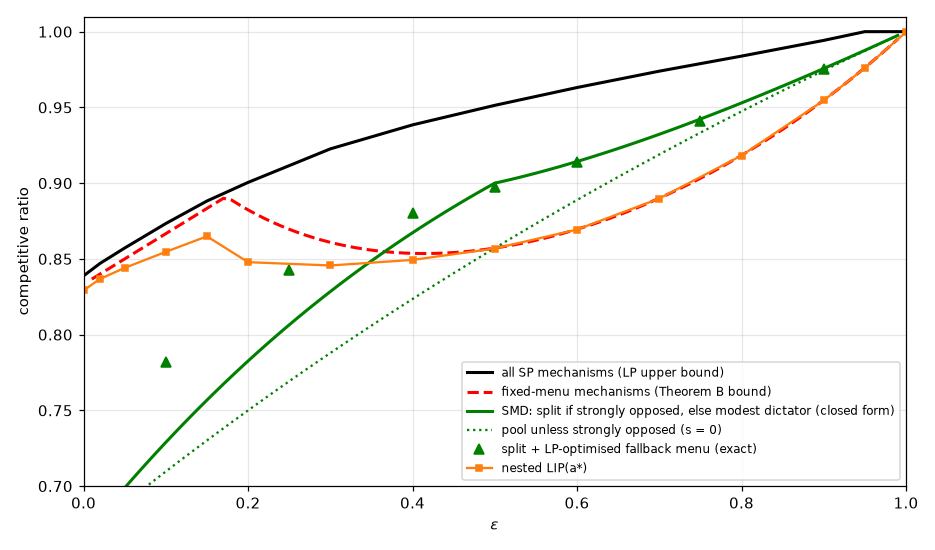
\includegraphics[width=0.75\linewidth]{../results/figures/04_beyond_dictatorship.png}
\caption{Complementarity model: LP upper bound on all strategy-proof mechanisms (black), the fixed-menu
bound of Theorem~B (red, dashed), nested LIP with optimised $a$ (orange), and the non-dictatorial SMD
mechanism of Propositions~D--E (green).}
\end{figure}

\paragraph{What remains open.} A strategy-proof mechanism approaching the LP bound for $0<\varepsilon<1$
(the LP-optimal mechanisms use smooth, type-dependent pooling probabilities); a closed form for the
$N\to\infty$ limit of the Theorem-1 LP; and whether any non-dictatorial mechanism beats $5/6$ in the
additive model (the LP suggests at most $\approx0.835$).
